
\chapter{Einleitung}
\thispagestyle{fancy}

\begin{quote}
This year’s Nobel Laureates are rewarded for having invented a new energy-efficient and environment-friendly light source – the blue light-emitting diode (LED). In the spirit of Alfred Nobel the Prize rewards an invention of greatest benefit to mankind; using blue LEDs, white Light can be created in a new way. \cite{nobelp} \end{quote}
\noindent
Dieser Satz, den die Schwedische Akademie der Wissenschaft nach der Vergabe des Nobelpreises an die Entwicklung der blauen LED (kurz, light emitting diode) im Jahr 2014 an die Presse veröffentlichte, fasst treffend zusammen, wie hoch die Bedeutung der auf Halbleiterkristallen basierenden optischen Bauelemente ist \cite{kneissl}. LEDs nehmen einen fundamentalen und immer bedeutender werdenden Teil unseres alltäglichen Lebens ein. Ausgezeichnet durch ihre hervorragende Effizienz, konkurrenzlosen Lebensdauer und geringen Dimension übernimmt sie durch eine immer höher werdende Lichtausbeute zusehends neue Anwendungsbereiche. Insbesondere auf Gallium Nitrid (GaN) basierende Halbleitermaterialien haben einen bahnbrechenden Weg hingelegt, der zur Entwicklung von hoch effizienten und leuchtstarken blauen LEDs führte und ebenfalls Grundlage für die Entwicklung in andere hochenergetische Wellenlängenbereiche darstellt \cite{risk} \cite{Shuji1999CandelaclassHI} \cite{10007979421}. So ebnet GaN auch den Weg für die Erzeugung von ultraviolett emittierenden Leuchtdioden. Der ultraviolette Spektralbereich, der sich in den UV-A (400 nm bis 320 nm), UV-B (320 nm bis 280) und UV-C Bereich (280 nm bis 200 nm) unterteilt, ist bedeutend für eine sehr hohe Anzahl spezieller Anwendungsbereiche. Beispielsweise bieten sich UV-LEDs an, um die bisher für Wasseraufbereitung genutzten Quecksilberdampflampen zu ersetzen \cite{Vilhunen2009}  \cite{WURTELE2011148}. Bislang werden für deren Betrieb Hochspannungsnetzteile verwendet, die einen mobilen Einsatz erheblich erschweren können. Hier bietet sich die Möglichkeit Abhilfe durch UV-LEDs zu verschaffen, da diese durch ihr kleines Format und durch die niedrigen Betriebsspannungen einen mobilen Einsatz ermöglichen. Ein weiteres Anwendungsgebiet ist die industrielle Aushärtung/Aufbrechung von Lacken und die Gasdetektion \cite{0268-1242-26-1-014036} \cite{LALINSKY2010152}. 
%
\begin{figure}[htb]
    \centering
    \begin{minipage}[t]{0.49\linewidth}
        \centering
        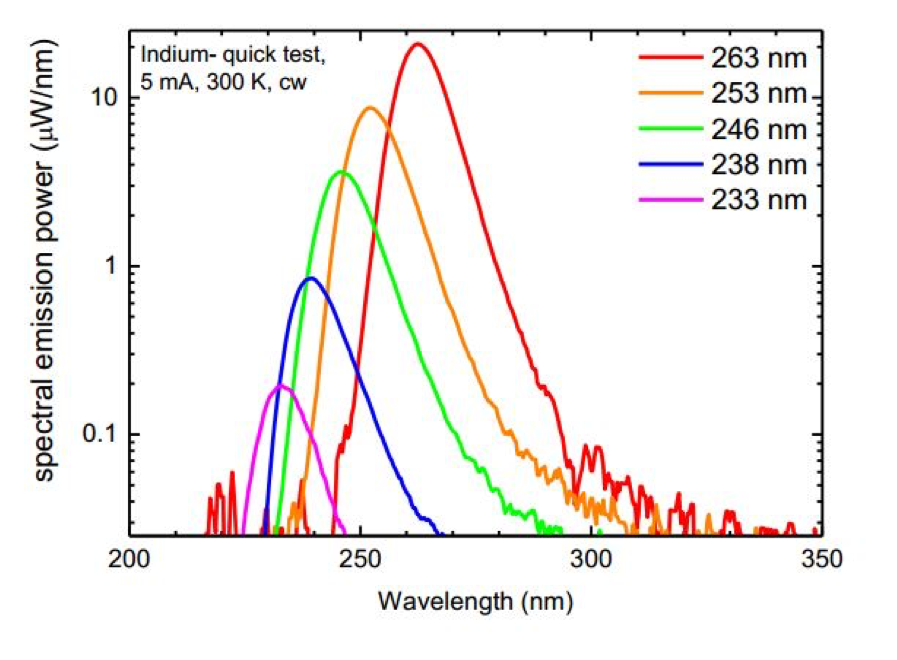
\includegraphics[width=\linewidth]{Bilder/SpectralEmissionPower_Wavelength.png}
        \caption{Spektrale Emissionsleistung für 5 verschiedene Wellenlängen von 263 nm bis 233 nm. Die Grafik zeigt, dass die spektrale Emissionsleistung mit sinkender Wellenlänge ebenfalls sinkt\cite{semreich}.}
        \label{fig:specPowWVL}
    \end{minipage}
    \hfill
    \begin{minipage}[t]{0.49\linewidth}
        \centering
        \includegraphics[width=\linewidth]{Bilder/Schichten.png}
        \caption{Aufbau einer LED-Heterostruktur mit vielen Schichten die unterschiedlichen Zwecken dienen.}
        \label{fig:schichtenLED}
    \end{minipage}
\end{figure}
\noindent
%
Für alle diese möglichen Applikationen ist eine hohe Ausgangsleistung notwendig. Aber wie in Abbildung \ref{fig:specPowWVL} zu sehen ist, sinkt die spektrale Emissionsleistung mit kleiner werdendem Wellenlängenbereich signifikant. Der Grund dafür ist, dass UV-LEDs bisher einer geringen Effizienz unterliegen, die quantitativ als Externe Quanteneffizienz (EQE) ausgedrückt wird und sich aus dem Produkt der internen Quanteneffizenz (IQE),Extraktions Effizenz (EE) und Injektionseffizienz (INJ) zusammensetzt:
%
\begin{equation}
    EQE = IQE \cdot EE \cdot INJ
\end{equation}
%
Die Gründe für die geringe Effizienz sind vielfältig. LEDs bestehen aus einer Vielzahl an Schichten (Abb. \ref{fig:schichtenLED}), die unterschiedlichen Funktionen dienen. Diese Schichten werden auf Substraten aufgewachsen. Eine hohe Substratqualität ist also der Grundbaustein für die optischen Eigenschaften und damit besonders entscheidend. Denn eine geringe Defektdichte im Substrat geht einher mit einer ebenfalls geringen Defektdichte in den aufgewachsenen Schichten und damit insbesondere der aktiven Zone, in der Elektronen und Löcher rekombinieren und Licht emittiert wird. Ein weiteres Problem im Zusammenhang mit den geringen Defektdichten ist ein Mangel an geeigneten Substratmaterialien. So wird aufgrund des Mangels an AlN-Substraten, beruhend auf den Schwierigkeiten bei der Herstellung, auf Saphir Substrate ausgewichen. Diese sind im fernen UV transparent und zusätzlich in großen Mengen in guter Qualität herstellbar. Problematisch jedoch ist die hohe Gitterfehlanpassung durch die relativ großen Unterschiede zwischen den Gitterkonstanten von AlN/GaN und Saphir. Durch diese sind AlN- und AlGaN-Schichten nicht vollverspannt aufwachsbar. Das führt dazu, dass die Schichten relaxieren, weil die Elastitizät der Schicht nicht groß genug im Vergleich zur Verspannungsenergie ist. Die Relaxation führt zur Entstehung von Versetzungen und Rissen. Diese agieren im Kristall als sogenannte nicht-radiative Rekombinationszentren, welche die IQE verringern. Die Hauptthematik dieser Arbeit liegt in der  Bestimmung der IQE von AlGaN - Heterostrukturen mit hohem Al-Gehalt mit Hilfe von temperatur- und leistungsdichteabhängigen Photolumineszenzmessungen.
So lässt sich bei der Annahme, dass bei Tieftemperatur keine nicht-strahlende Rekombination stattfindet, die IQE als Quotient der Intensität der Photolumineszenz bei Tieftemperatur (5K) und Raumtemperatur (300K) beschreiben.  
Das Kapitel \ref{chap:mqw} widmet sich der Untersuchung von AlGaN-MQWs verschiedener Dicken mit dotierten und undotierten Barrieren. Mit Hilfe von temperaturabhängiger UV-Photolumineszenzmessungen wird der Einfluss des QCSE auf die IQE experimentell ermittelt um eine optimale MQW-Struktur zu bestimmen.
In \ref{chap:offcut} wird der Einfluss des Fehlschnittwinkels des Substrates auf die IQE untersucht. Dieser nimmt deutlichen Einfluss auf die Wachstumskinetik und somit auf die Anordnung der monoatomaren Schichten und zeigt sich insbesondere an der Oberflächenmorphologie, auf die im Kapitel im Speziellen mit Hilfe verschiedener Messmethoden eingegangen wird.
In Kapitel \ref{chap:pol} werden theoretische Simulationen der Polarisation für AlGaN experimentell überprüft. Die Polarisation hat bedeutenden Einfluss auf die Extraktionseffizienz (EE) und somit auf die EQE.
Im letzten Kapitel der Arbeit wird eine Methode analysiert, die eine Möglichkeit beschreibt, durch leistungsdichteabhängige Messungen bei Raumtemperatur die IQE zu bestimmen. Das ist insofern ein Vorteil, dass ein aufwendiges Runterkühlen auf 5K nicht notwendig ist. 













